\chapter{Applications}

\section{Power-law noise}

The statistical test mentioned in the previous chapter is tested on computer-generated power-law noise series.\cite{Timmer1995} the $\beta$ term in the formula $\frac{1}{f^{\beta}}$ will be referenced ask for the rest of the paper. Three values of k are chosen: $k_1=(1,3,5)$. For each $k_1$ value, another set of k values is generated using the formula $k_2=(k_1-e^0,k_1-e^{-1},k_1-e^{-2},k_1-e^{-3},k_1+0,k_1+e^0,k_1+e^{-1},k_1+e^{-2},k_1+e^{-3})$. The statistical test is used on every possible pair of a value from $k_1$ and a value from $k_2$. Two power-law series are generated using each value in the pair. The series has 1,000 elements. The hypothesis will be rejected if the p-value is less than 0.05. 10 iterations are done for each pair. A plot will be made for each $k_1$ value of the rejection rate of the statistical test. A NaN plot is included for each plot, which shows the rate, at which the statistical test produces NaN values. NaN values are only produced in the last graph. Power-law series with k=5 have entropy around $0.4$, the rest of the time series that will be examined in the paper have entropy above 0.9, so this should not be a problem. The Rejection plot for $k_1=1$ is quite surprising in the sense that many values around $k_1$ has a high rejection rate. $k_1=3$ looks the most as, what was expected since the further away a point gets from $k_1$ the larger is the rejection rate.



\begin{figure}
    \centering
    \begin{subfigure}[b]{0.3\textwidth}
        \centering
        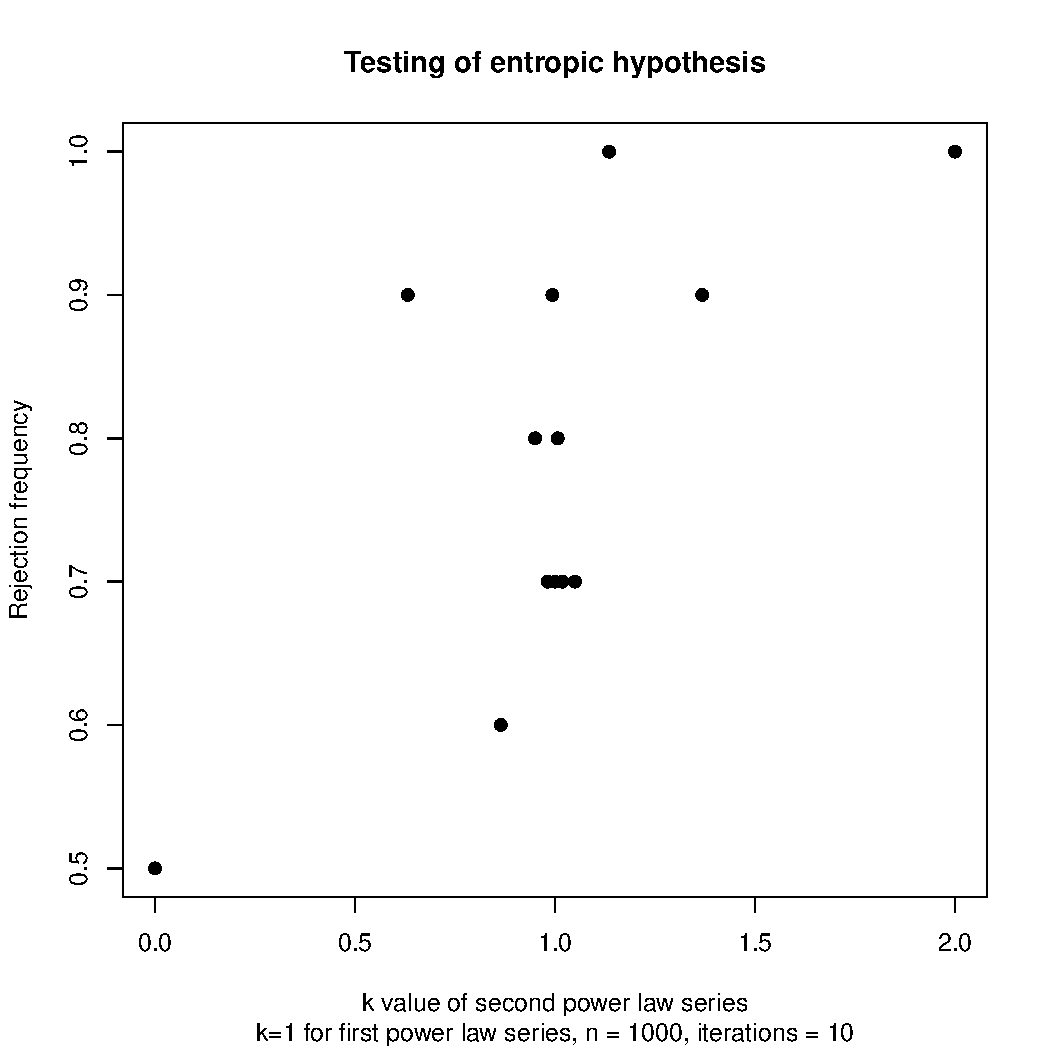
\includegraphics[height=7cm,keepaspectratio]{./powerlaw/rejectionPlot,k1=1,n=1000,iterations=10.pdf}
        % This plot was produced with lines XXX of file YYY; increase the legend size, use serif fonts
    \end{subfigure}
    \hfill
    \begin{subfigure}[b]{0.5\textwidth}
        \centering
        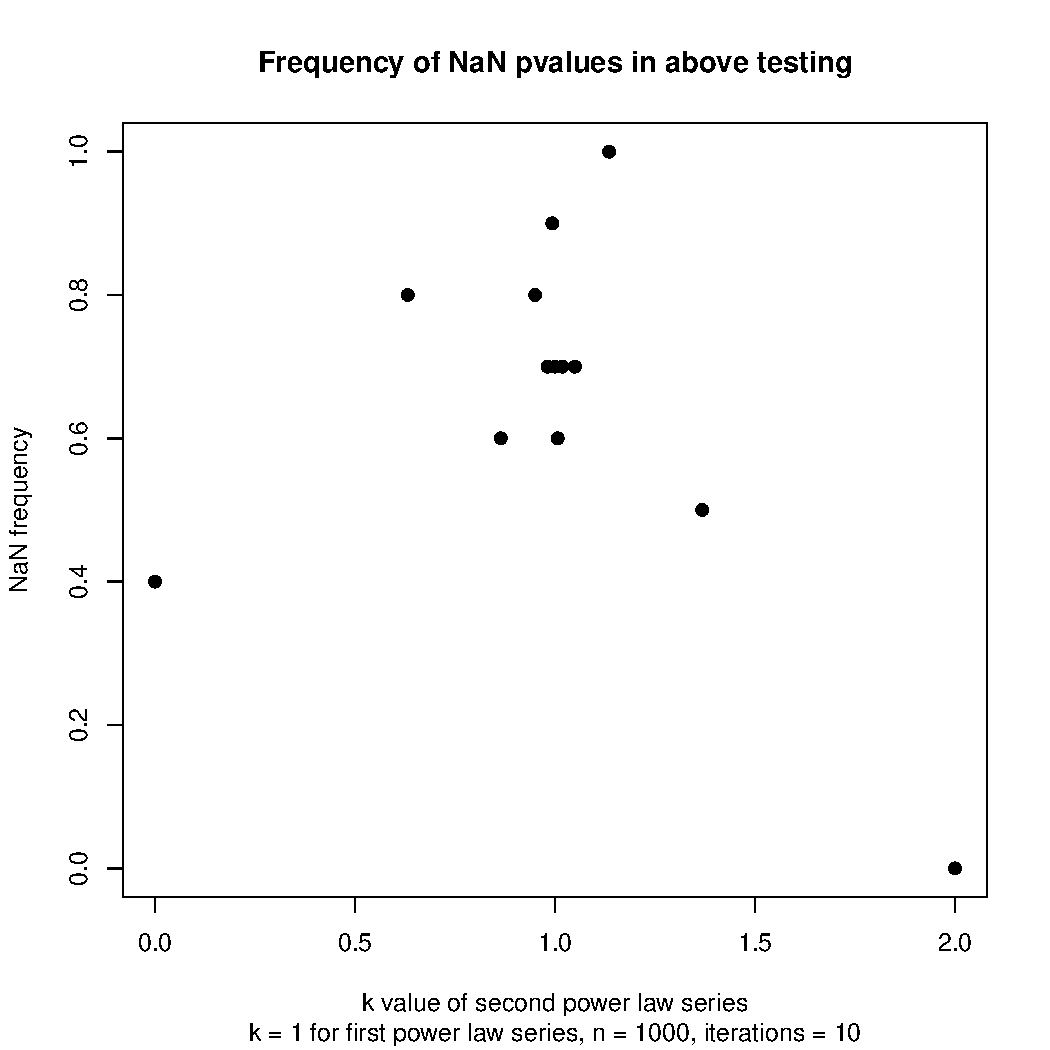
\includegraphics[height=7cm,keepaspectratio]{./powerlaw/NaNPlot,k1=1,n=1000,iterations=10.pdf}
    \end{subfigure}
    \vfill
    \begin{subfigure}[b]{0.3\textwidth}
        \centering
        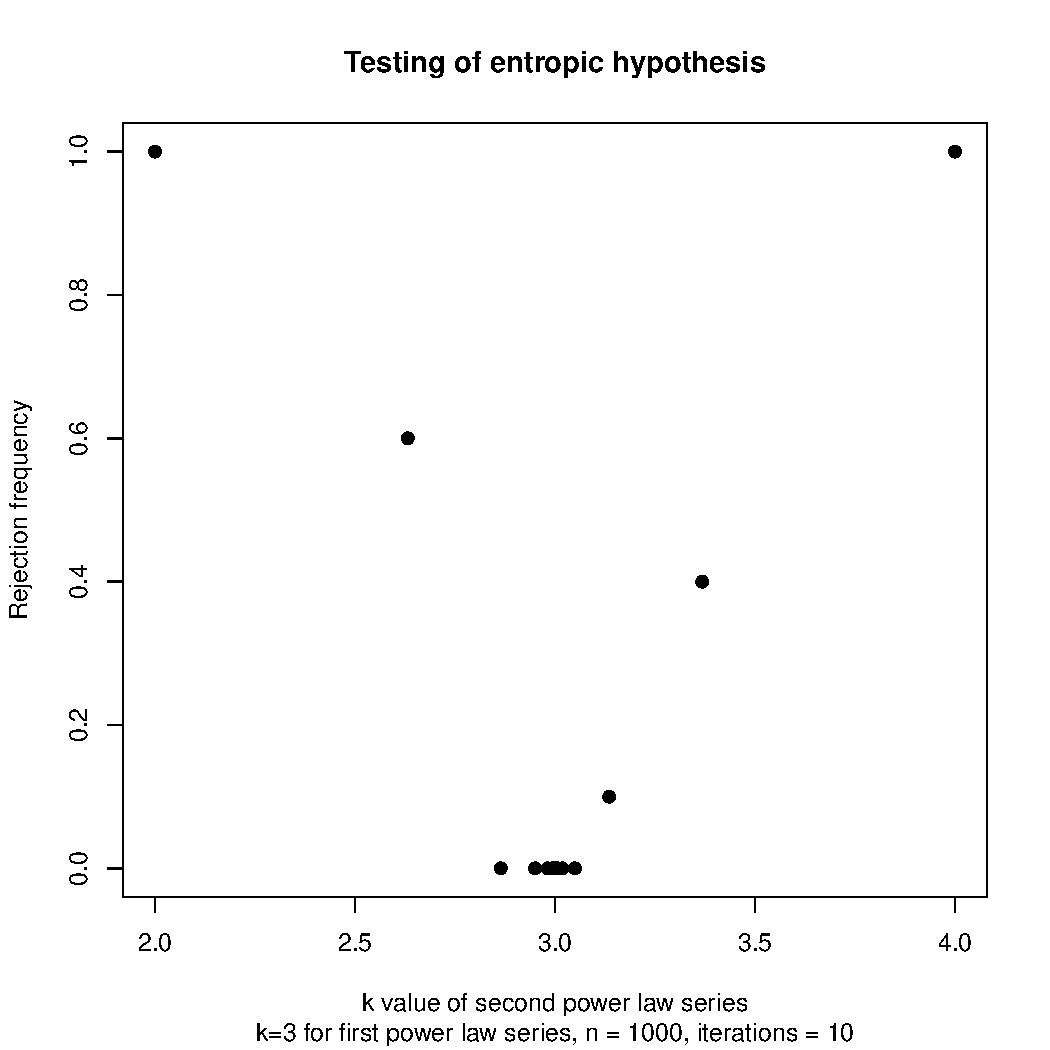
\includegraphics[height=7cm,keepaspectratio]{./powerlaw/rejectionPlot,k1=3,n=1000,iterations=10.pdf}
    \end{subfigure}
    \hfill
    \begin{subfigure}[b]{0.5\textwidth}
        \centering
        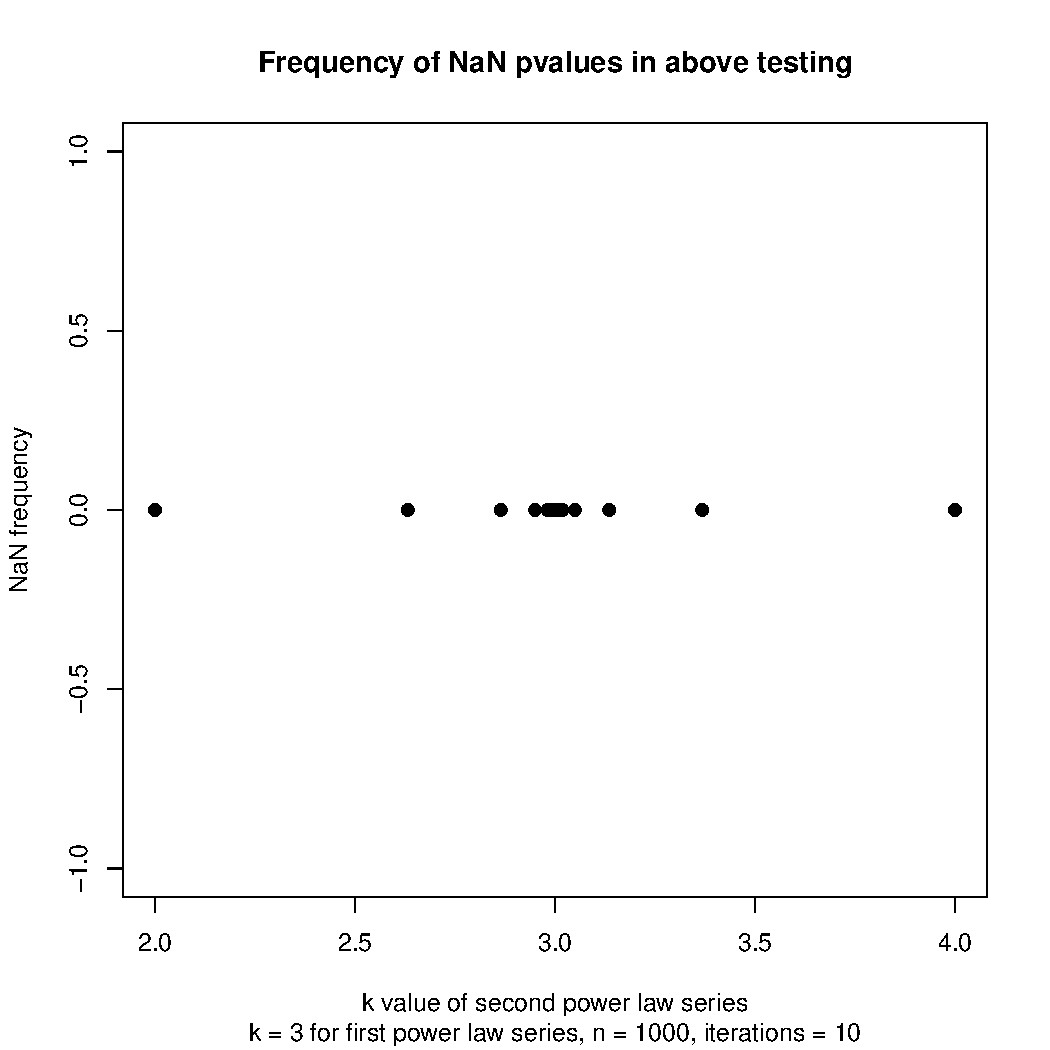
\includegraphics[height=7cm,keepaspectratio]{./powerlaw/NaNPlot,k1=3,n=1000,iterations=10.pdf}
    \end{subfigure}
    \vfill
    \begin{subfigure}[b]{0.3\textwidth}
        \centering
        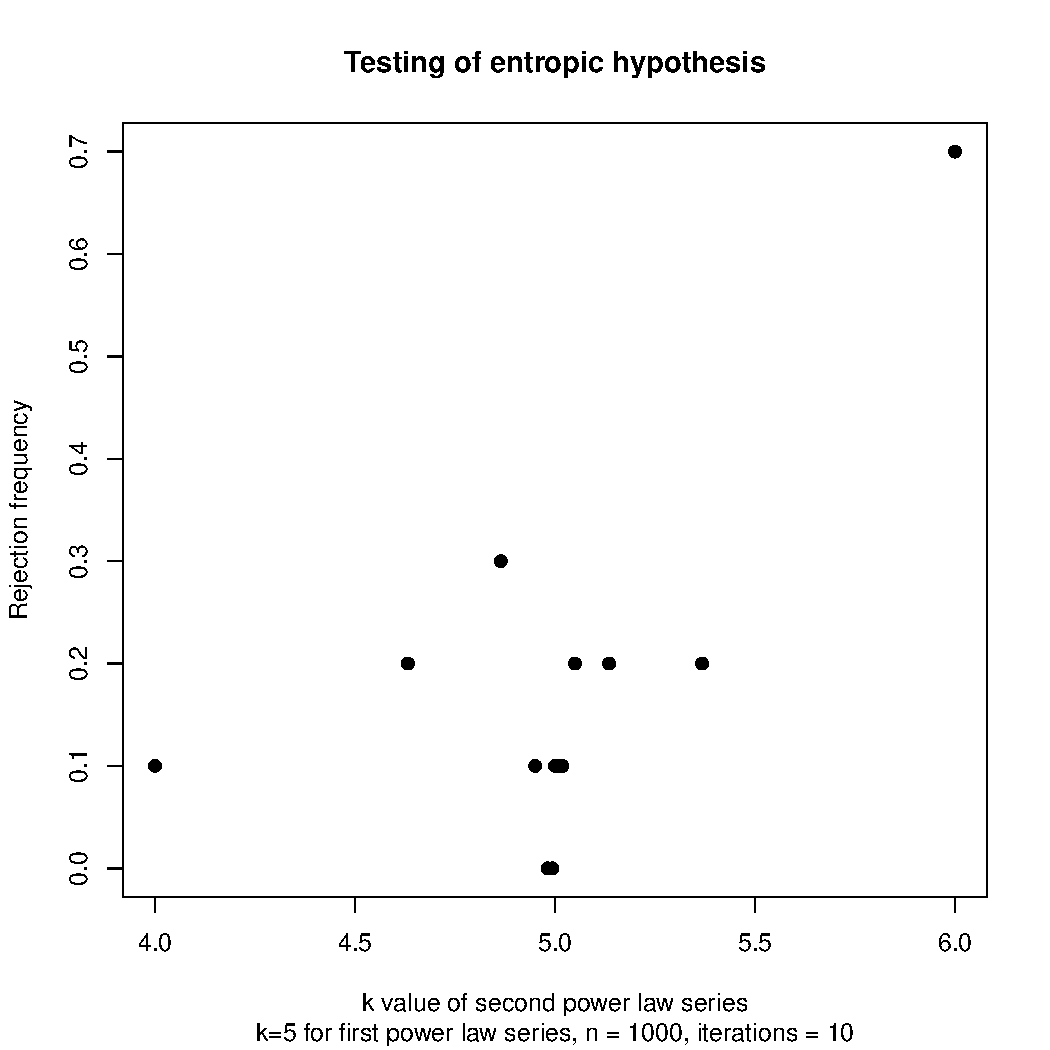
\includegraphics[height=7cm,keepaspectratio]{./powerlaw/rejectionPlot,k1=5,n=1000,iterations=10.pdf}
    \end{subfigure}
    \hfill
    \begin{subfigure}[b]{0.5\textwidth}
        \centering
        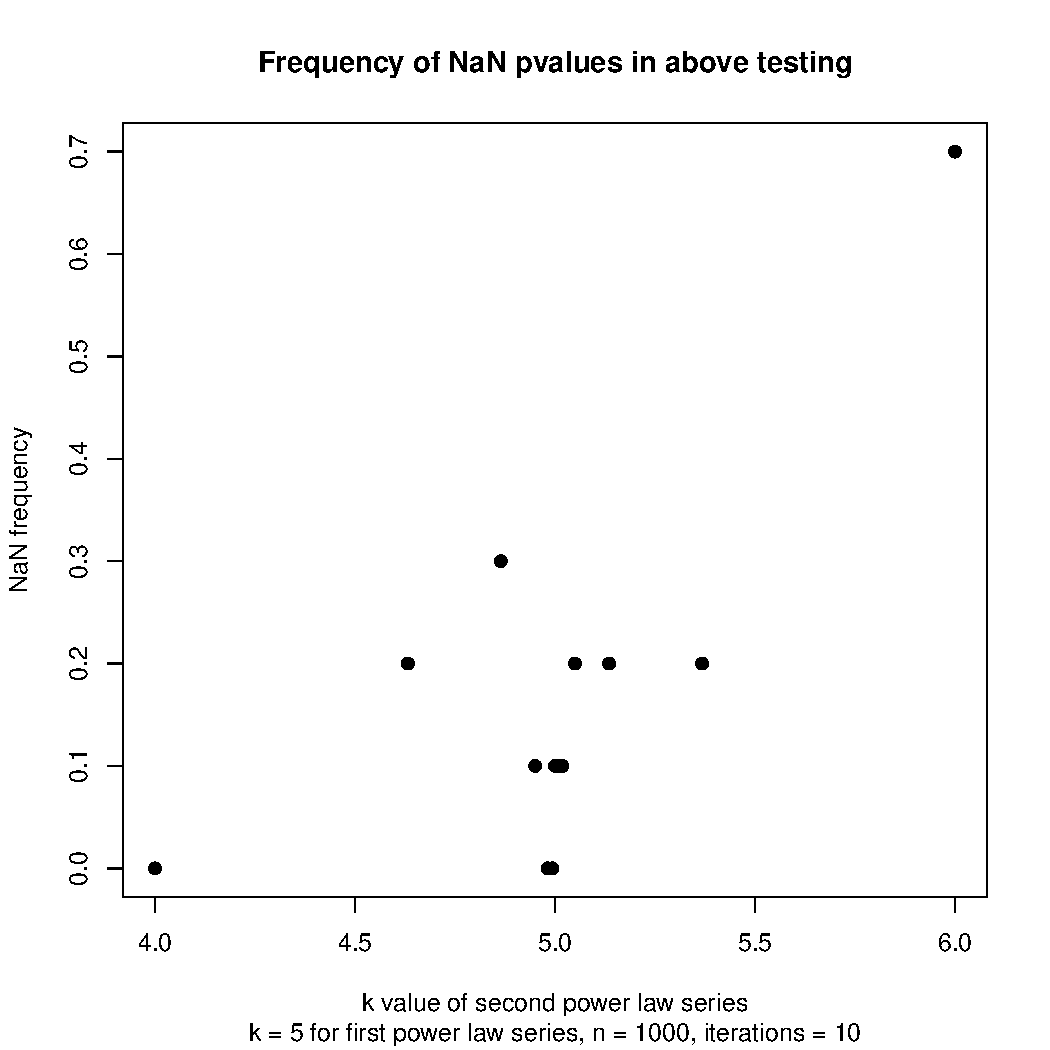
\includegraphics[height=7cm,keepaspectratio]{./powerlaw/NaNPlot,k1=5,n=1000,iterations=10.pdf}
    \end{subfigure}
    \caption{Power-law experiment}
\end{figure}

\FloatBarrier

\section{Idea behind new tie breaking}
In the next section, a new way to break ties will be implemented and used. The idea behind it is when having a tie, instead of either randomly assigning it to any of the possible patterns, which was proposed by Bandt and Pompe in their original paper~\cite{Bandt2002}, or always assigning a type of tie to a given pattern, which is done in the article being used in the next section~\cite{Chagas2022}, the new idea is to assign an equally large weight to all the possible patterns in case of a tie. In a tie, with k possible patterns, each of these k patterns gets a weight of $\frac{1}{k}$. The amount of possible patterns is the product of the occurrence of each unique value. To calculate the ordinal pattern distribution, simply sum up all the weights for each pattern and divide by the total amount of weight to get the frequency. Ordinal patterns are often used in fields that do science on real-world phenomena. In cases where the measuring equipment has a low precision, ties will often occur, e.g. a weight measurement. It is commonly known that objects have an atomic weight, since all everyday objects are made of particles that have an atomic weight. The atomic weight unit is $1\mu = 1.66..\cdot10^{-27}kg$, so the theoretical weight of an object has a lot of decimals, which could theoretically be measured, however putting a person on a normal household scale will only give a result in kilograms with one decimal. A person measuring themselves on a scale at different times and weighing the same does not mean they had the same atomic weight at both times. Their data would result in a tie, but based on the above argumentation it is fair to assume that in reality, the weight has either gone up or down, however, it is impossible with the given instruments to measure, which it is, so the only fair assumption is that both cases are equally likely. This can almost be seen as superposition\cite{Schroedinger1926} of the change of weight. The weight has gone both up and down until a more precise measurement is made, but until that, it is only fair to think both cases are possible and in this case equally possible. This type of tie-breaking should work, where it can be argued that a theoretical measurement has a higher precision than the actual measurement. It does, however, not make sense to use it, when the measured value can be argued to be of the same precision as a theoretical measurement, e.g. “How many cows are in front of me at a certain type?”. This implementation will briefly be referenced as “My implementation”, but mostly as a “Theoretical Split”. Note that the theoretical split method does not need noise added. Adding noise removes all ties, which means it should perform identically to “article implementation”, which is the implementation made in the article\cite{Chagas2022}, since it is built upon that code. The theoretical split and the second tie-breaking solution are deterministic, whereas the Bandt and Pompe solution is stochastic.

\FloatBarrier

\section{Temperature Data}
\cite{Chagas2022} Will be partly reproduced and additional plots and tables will be made. Only the maximum temperature part of the climate data in section 6 of the article will be used. As can be seen in Figure 4.2 the percentage of ties in this dataset is extremely high. It is therefore quite important, how ties are handled since they make up a bulk of the dataset. 
\begin{figure}
    \centering
    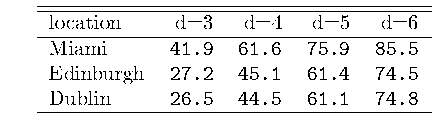
\includegraphics{./Weather/tiesTable.pdf}
    \caption{Table of ties in percentage}
\end{figure}


The libraries mentioned earlier all handle ties differently, as seen in Figure 4.3. The first three columns are the setting of each experiment. The start date column is included, because the paper, where the data is from, accidentally started their data on 1992-08-14, instead of 1992-08-08 as they said the data started from, it does however not make a big difference, which can be seen between the top three rows and bottom three rows.  If all the values in a row are identically, that means the libraries perform identically. The only setting, where this happens, is when noise is added and Na values are omitted. Na omit removes Na values and the dataset is pushed together, where the Na values have been removed. In the rest of the experiment, this setting will be used. 

\begin{figure}
    \centering
    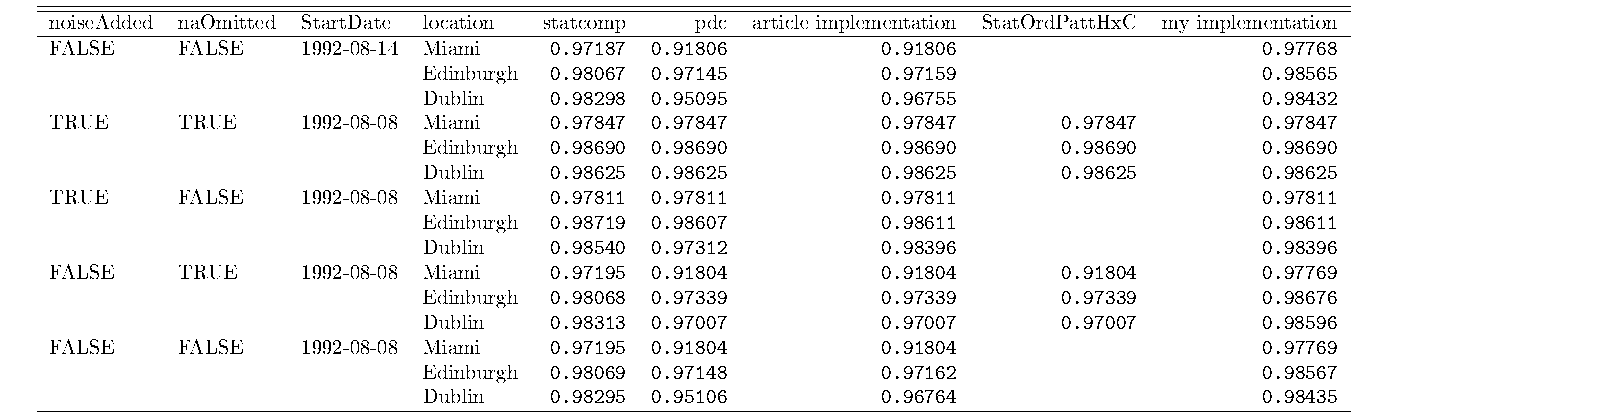
\includegraphics[width=\textwidth,keepaspectratio]{./Weather/entropyTable.pdf}
    \caption{Entropy table of libraries performs on different preprocessing}
\end{figure}

A more in-depth analysis of the Theoretical Split versus adding noise is made. The statcomp library is the comparison library, but it does not matter, which library is chosen, since they perform identically in this case. As can be seen in Figure 4.5 the theoretical value is very close to both the mean and median of the entropy of 1,000 iterations. Figure 4.4 clearly shows the problem of adding a random sample of white noise, since the value might easily end up 0.001 off either the mean, median, or theoretical value, which all seem to be quite precise values of the entropy since the theoretical value is calculated quite differently then the mean and median, but they still end up much closer, then a random sample do. 

\begin{figure}
    \centering
    
\includegraphics[width=\textwidth,keepaspectratio]{./Weather/noiseStochasticTheoretical.pdf}
    \caption{Iterations of adding noise vs theoretical split in sorted order, the vertical line is median and horizontal is theoretical split value.}
\end{figure}

\begin{figure}
    \centering
    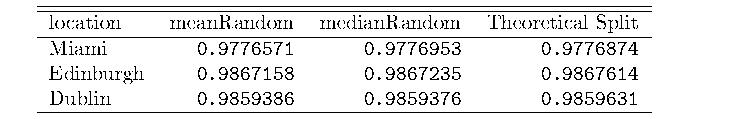
\includegraphics[width=\textwidth,keepaspectratio]{./Weather/random_vs_theoreticalSplit.pdf}
    \caption{Table of mean and median of adding noise and theoretical split. Temperature dataset}
\end{figure}

The above experiment is repeated, but where the theoretical split is fed a constant dataset. The constant values here represent very imprecise measurements, where the true values of the observed phenomenon are assumed to be different. E.g. trying to measure white noise, with a bad instrument. It is important to note that if a dataset contains just a single constant value, where the measurement is precise. The entropy would naturally be 0, since there is full predictability, e.g. “how many cows are on the field at a given time”. The iterations are calculated on random numbers, which ideally should be white noise. Figure 4.6 rarely has the entropy of ideal white noise, which is 1, where the theoretical split can correctly calculate that the poorly measured white noise has entropy 1. Figure 4.7 shows that the median measurement is closer than the mean to the theoretical split, so it might be a better measurement. In Figure 4.5 the median is generally also closer to the theoretical split. The median has another benefit over the mean, in the fact that it might not always be mathematically true to take the mean of an approximation, where the median is an entropy generated by an actual time series.

\begin{figure}
    \centering
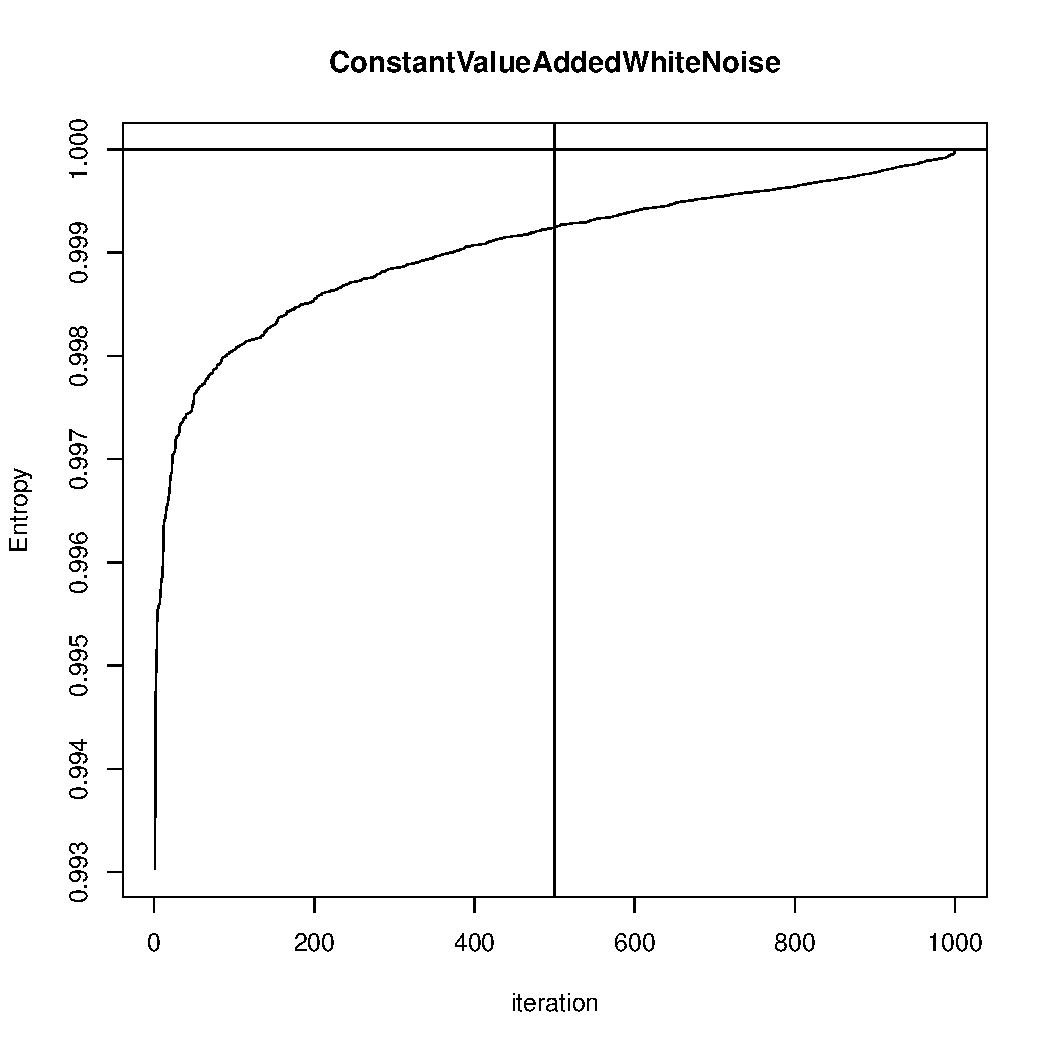
\includegraphics[width=\textwidth,keepaspectratio]{./Weather/constantWithWhiteNoiseStochasticTheoretical.pdf}
    \caption{Constant dataset}
\end{figure}

\begin{figure}
    \centering
    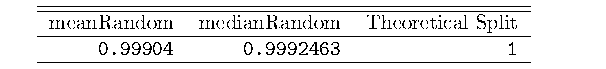
\includegraphics[width=\textwidth,keepaspectratio]{./Weather/random_vs_theoreticalSplitWhiteNoise.pdf}
    \caption{Mean and median of adding noise and theoretical split, constant dataset.}
\end{figure}

Figure 4.8 is a plot of the theoretical split values as the entropy of the three locations on the HxC plane, with confidence intervals on the entropy. At first glance, it looks like the confidence interval sticks out of the boundaries, however it is important to remember that a change in entropy leads to a change in complexity, so the confidence intervals are not breaking the boundaries. 

\begin{figure}
    \centering
    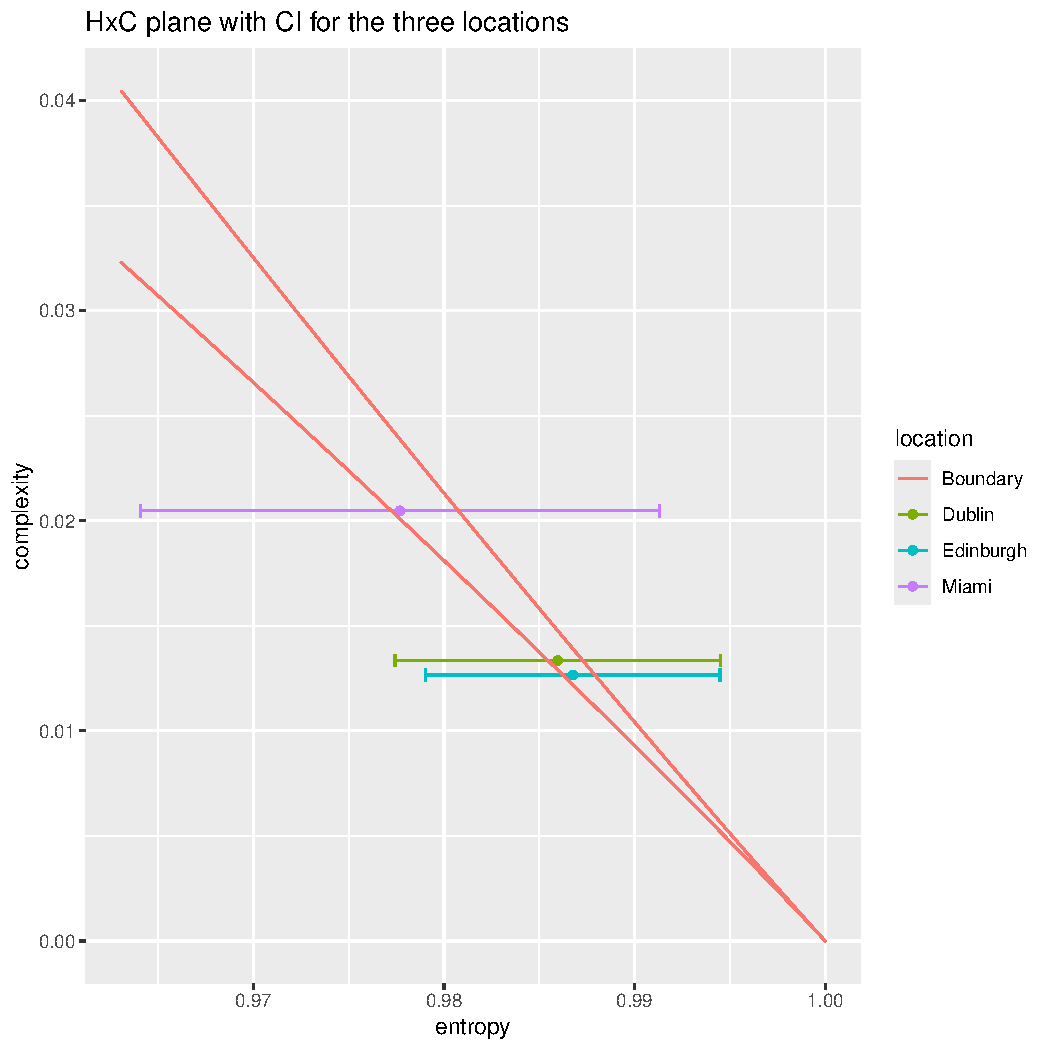
\includegraphics[width=\textwidth,keepaspectratio]{./Weather/confidenceIntervalPlot.pdf}
    \caption{HxC plane of locations with confidence interval}
\end{figure}

P values are calculated. 10 iterations are done on adding noise for breaking ties and compared with the p-value of the theoretical split. The theoretical p value is only larger than one iteration for Miami-Edinburgh, two for Miami-Dublin and four for Edinburgh-Dublin, which is OK. Ideally, it should be between iteration 5 and 6. Most importantly, it is the range of the iterations, which definitely confirms it is implemented so what correctly. 


Adding noise has a couple of problems in the sense that it is much more computer-intensive to calculate just 10 iterations compared with the theoretical value once.
'\begin{figure}
    \centering
    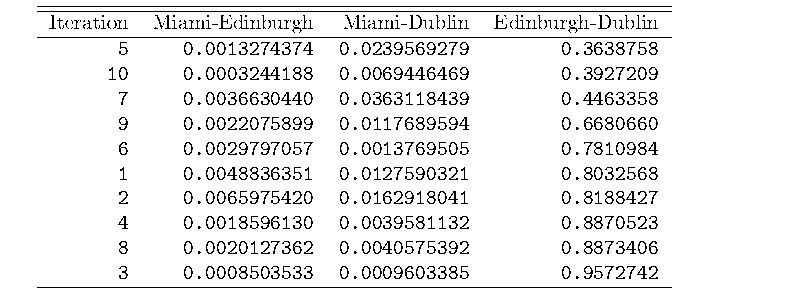
\includegraphics[width=\textwidth,keepaspectratio]{./Weather/pValuesTheoretical,10=Iterations,Sorted.pdf}
    \caption{Noise added, 10 iterations, sorted by column “Edinburgh-Dublin"}
\end{figure}

'\begin{figure}
    \centering
    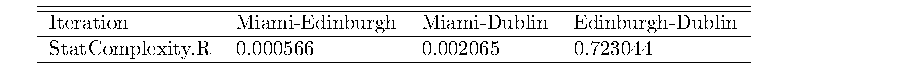
\includegraphics[width=\textwidth,keepaspectratio]{./Weather/pValuesTheoretical.pdf}
    \caption{p value, when using theoretical split}
\end{figure}

